\scanpage{108}
\mspage{107}%
motives over $\underline{C}$ in fact takes its values in the category of Hodge structures (a polarization of a smooth projective variety $V$ canonically defines a polarization of the associated Hodge structure on Betti-Hodge cohomology). NB One has no idea what the essential image of the preceding functor might be, for example whether there is reason to hope that one finds all Hodge structures (hence an equivalence of categories : motives over $\underline{C}$ $\handwritten{\longrightarrow}$ Hodge structures); this seems unlikely, but one has no serious indication one way or the other.

The category of \deleted{pre} Hodge structures is semi-simple. \deleted{In fact,} If $G$ is the Galois group of a \inserted{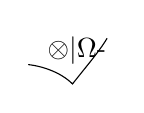
\begin{tikzpicture}[baseline=-.2ex,x=1em,y=1em]
\node[anchor=base west] at (0,.45) {$\unsure{\otimes|\Omega}$-};
\draw (-.35,.2) .. controls (.1,.15) and (.8,-.05) .. (1.25,-.5) .. controls (1.8,.2) and (2.2,.65) .. (2.5,1.15);
\end{tikzpicture}}category \inserted{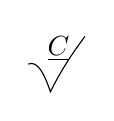
\begin{tikzpicture}[baseline=-.2ex,x=1em,y=1em]
\node[anchor=base west] at (0,.5) {$\underline{C}$};
\draw (-.35,.2) .. controls (0,.35) and (.25,-.2) .. (.45,-.8) .. controls (.75,-.2) and (1.1,.4) .. (1.7,1.2);
\end{tikzpicture}} of pre-Hodge structures, finitely generated if one wishes (to simplify), then one can make explicit in terms of the associated Galois group and of it\deleted{\unsure{e}}s\deleted{s} structure\deleted{s} $i_1\deleted{,\unsure{i_2}}$ above the condition \deleted{that} for the objects of $\underline{C}$ to be in fact Hodge structures. This is a pleasant and delectable exercise, which should appear in a systematic work on $\otimes$-categories, in the chapter of examples. One finds very serious restrictions on the group $G$ \deleted{(plus} equipped with $i_1$ (in addition to the fact that $G$ is reductive).

4) I leave it to Saavedra to determine what additional structure one obtains on the ``complex'' Hodge structure associated with a \inserted{
\begin{tikzpicture}[baseline=-.2ex,x=1em,y=1em]
\node[anchor=base west] at (0,.5) {smooth};
\draw (.1,-.7) .. controls (.2,-.25) and (.5,.1) .. (1,.15) .. controls (2.3,.25) and (3.3,.25) .. (3.5,.5) -- (3.55,.9);
\end{tikzpicture}} complex projective variety $X$, when the latter is given as obtained from a real project\rlap{\raisebox{1.1ex}{\tikz[x=1em,y=1em]{\draw (0,0)--(0,.12) (0,.2)--(.01,.33) (.01,.43)--(.02,.49);}}}ive variety $X_{\underline{R}}=X_o$.One finds a notion of ``real Hodge structure'', giving rise to a corresponding $\otimes$-category. In the motivic Galois group of the latter, in addition to the structure $i_1$, one finds an element $f_{\handwritten{\infty}}$ of $G(\underline{Q})$, \deleted{of degree} of order 2 (playing the role of a ``\rlap{f}Frobenius element at infinity''), which corresponds \margin{\tikz[x=1em,y=1em]{\draw (0,0) .. controls (.08,.02) and (.15,.13) .. (.2,.25);}}to the automorphism of the Betti functor $X_o\handwritten{\longmapsto} H^{\handwritten{*}}(X_o(\underline{C}),\underline{Q})$ induced by the homeomorphism $x\handwritten{\mapsto}\overset{\handwritten{\rule{.55em}{.35pt}}}{x}$ of $X_o(\underline{C})$. One must make explicit the relations between this element and $i_1$, $i_2$ !
